\subsubsection{Convection in a box with prescribed, variable velocity boundary conditions}
\label{sec:cookbooks-platelike}

A similarly simple setup to the ones considered in the previous subsections is
to equip the model we had with a different set of boundary conditions. There, we used slip boundary
conditions, i.e., the fluid can flow tangentially along the four sides of our
box but this tangential velocity is unspecified. On the other hand, in many
situations, one would like to actually prescribe the tangential flow velocity as
well. A typical application would be to use boundary conditions at the top that
describe experimentally determined velocities of plates. This cookbook shows a
simple version of something like this. To make it slightly more interesting, we
choose a $2\times 1$ domain in 2d.

Like for many other things, \aspect{} has a set of plugins for prescribed
velocity boundary values (see
Sections~\ref{parameters:Boundary_20velocity_20model} and
\ref{sec:prescribed-velocity-boundary-conditions}). These plugins allow one to
write sophisticated models for the boundary velocity on parts or all of the
boundary, but there is also one simple implementation that just takes a formula
for the components of the velocity.

To illustrate this, let us consider the \url{cookbooks/platelike-boundary/platelike-boundary.prm}
input file. It essentially extends the input file considered in the previous example.
The part of this file that we are particularly interested in in the current
context is the selection of the kind of velocity boundary conditions on the four
sides of the box geometry, which we do using a section like this:
\lstinputlisting[language=prmfile]{boundary.part.prm.out}

We use tangential flow at boundaries named left, right and bottom.
Additionally, we specify a comma separated list (here with only a single
element) of pairs consisting of the name of a boundary and the name of a
prescribed velocity boundary model. Here, we use the \texttt{function} model on
the \texttt{top} boundary, which allows us to provide a function-like notation
for the components of the velocity vector at the boundary.

The second part we need is that we actually describe the function that sets the
velocity. We do this in the subsection \texttt{Function}. The first of these
parameters gives names to the components of the position vector (here, we are
in 2d and we use $x$ and $z$ as spatial variable names) and the time. We could
have left this entry at its default, \texttt{x,y,t}, but since we
often think in terms of ``depth'' as the vertical direction, let us use
\texttt{z} for the second coordinate.
In the second parameter we define symbolic constants that can be used
in the formula for the velocity that is specified in the last parameter. This
formula needs to have as many components as there are space dimensions,
separated by semicolons. As stated, this means that we prescribe the
(horizontal) $x$-velocity and set the vertical velocity to zero. The horizontal
component is here either $1$ or $-1$, depending on whether we are to the right
or the left of the point $1+\sin(\pi t/2)$ that is moving back and forth with
time once every four time units. The \texttt{if} statement understood by the
parser we use for these formulas has the syntax
\texttt{if(condition, value-if-true, value-if-false)}.

\note{While you can enter most any expression into the parser for these
velocity boundary conditions, not all make sense. In particular, if you use an
incompressible medium like we do here, then you need to make sure that either
the flow you prescribe is indeed tangential, or that at least the flow into and
out of the boundary this function applies to is balanced so that in sum the
amount of material in the domain stays constant.

It is in general not possible for \aspect{} to verify that a given input is
sensible. However, you will quickly find out if it isn't: The linear solver for
the Stokes equations will simply not converge. For example, if your function
expression in the input file above read \\
\hspace*{.25cm} \texttt{if(x>1+sin(0.5*pi*t), 1, -1); 1}\\
then at the time of writing this you would get the following error message: \\
\hspace*{.25cm}\texttt{*** Timestep 0:  t=0 seconds} \\
\hspace*{.25cm}\texttt{   Solving temperature system... 0 iterations.} \\
\hspace*{.25cm}\texttt{   Rebuilding Stokes preconditioner...} \\
\hspace*{.25cm}\texttt{   Solving Stokes system... } \\
\\
\hspace*{.25cm}\texttt{\ldots some timing output \ldots} \\
\\
\\
\hspace*{.25cm}\texttt{----------------------------------------------------} \\
\hspace*{.25cm}\texttt{Exception on processing: } \\
\hspace*{.25cm}\texttt{Iterative method reported convergence failure in step
9539 with residual 6.0552} \\
\hspace*{.25cm}\texttt{Aborting!} \\
\hspace*{.25cm}\texttt{----------------------------------------------------}

The reason is, of course, that there is no incompressible (divergence free) flow
field that allows for a constant vertical outflow component along the top
boundary without corresponding inflow anywhere else.}


The remainder of the setup is described in the following, complete input file:
\lstinputlisting[language=prmfile]{platelike.prm.out}


This model description yields a setup with a Rayleigh number of 200 (taking
into account that the domain has size 2). It would, thus, be dominated by heat
conduction rather than convection if the prescribed velocity boundary conditions
did not provide a stirring action. Visualizing the results of this simulation%
\footnote{In fact, the pictures are generated using a twice more refined mesh
to provide adequate resolution. We keep the default setting of five
global refinements in the parameter file as documented above to keep compute
time reasonable when using the default settings.}
yields images like the ones shown in Fig.~\ref{fig:platelike}.

\begin{figure}
  \centering
  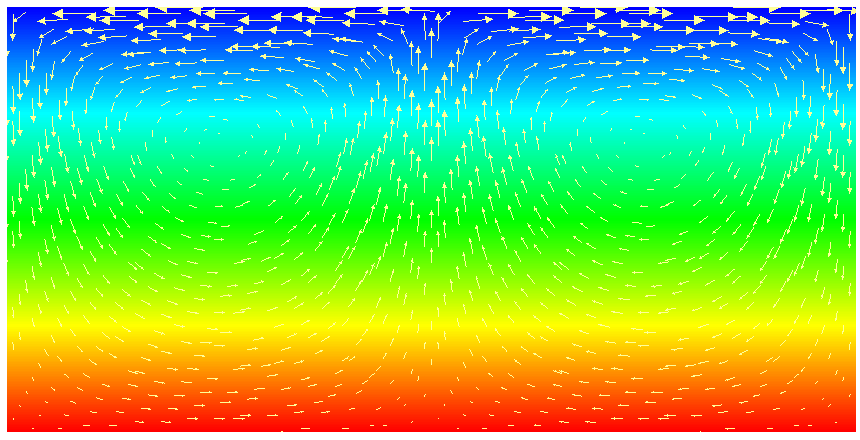
\includegraphics[width=0.3\textwidth]{visit0000.png}
  \hfill
  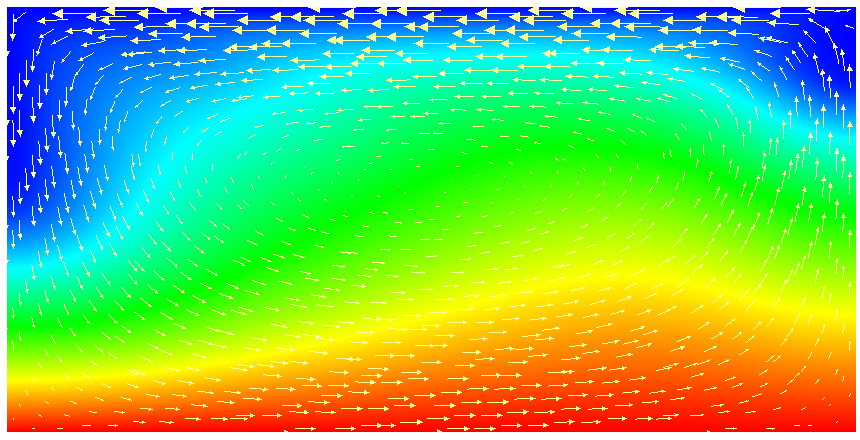
\includegraphics[width=0.3\textwidth]{visit0001.png}
  \hfill
  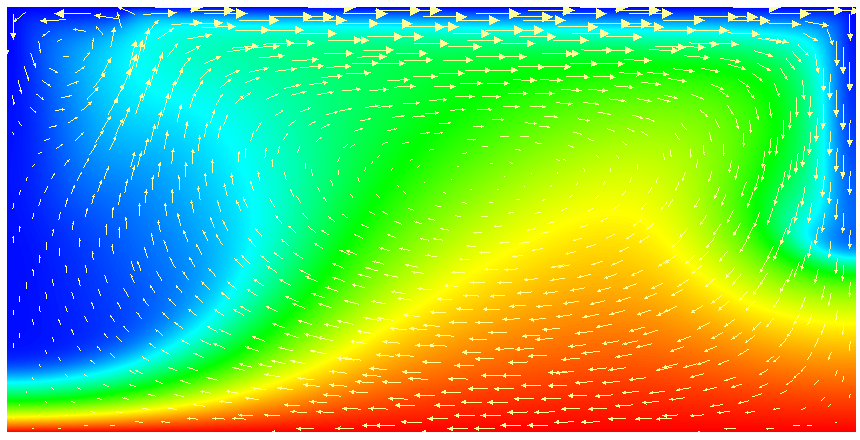
\includegraphics[width=0.3\textwidth]{visit0003.png}
  \\
  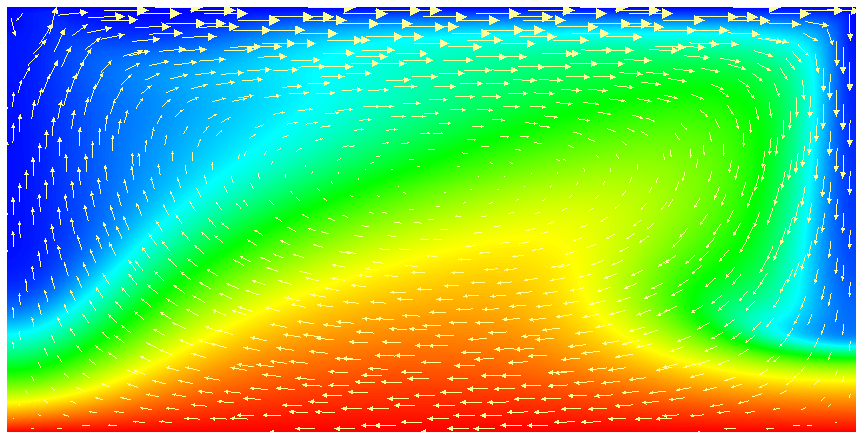
\includegraphics[width=0.3\textwidth]{visit0004.png}
  \hfill
  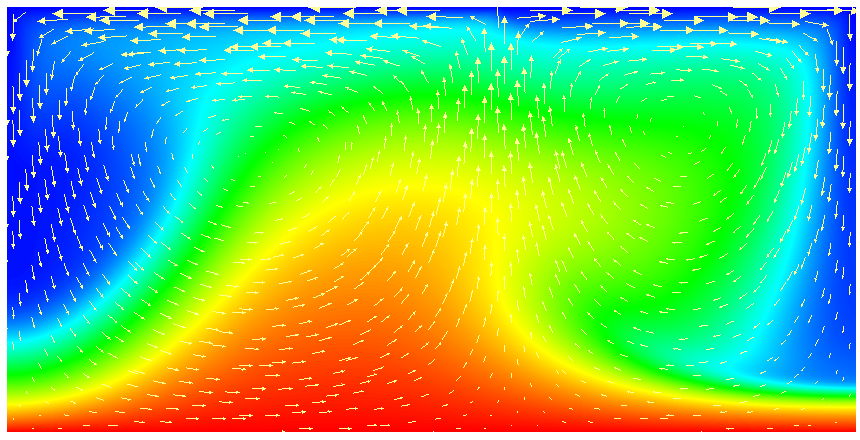
\includegraphics[width=0.3\textwidth]{visit0005.png}
  \hfill
  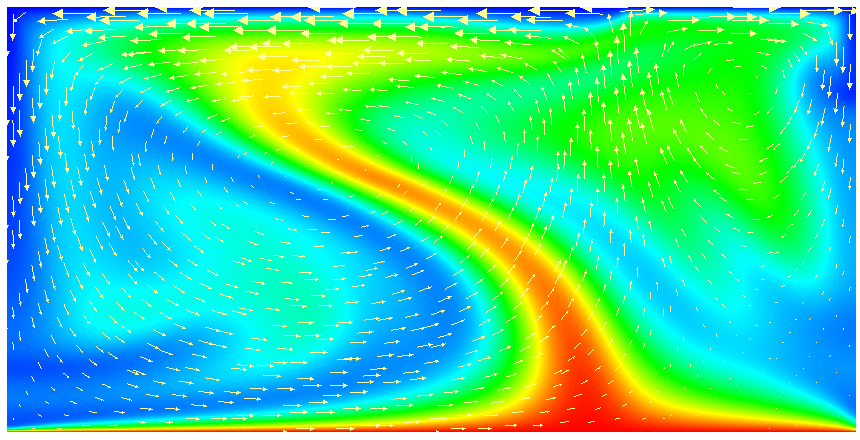
\includegraphics[width=0.3\textwidth]{visit0006.png}
  \caption{\it Variable velocity boundary conditions: Temperature and velocity
  fields at the initial time (top left) and at various other points in time during the
  simulation.}
  \label{fig:platelike}
\end{figure}


